\documentclass[../main.tex]{subfiles}
\usepackage{graphicx}

\begin{document}
\textbf{Component 3: Individual Questions (SW Development)}
\newline
\newline
\textbf{What technical or professional skills have you identified were relevant to the project?}
\newline
\newline
Full-stack development was important in creating the Collaborative Disaster Response System, enabling a seamless experience for emergency responders, volunteers, and affected communities[11]. I worked on both the frontend (React.js) and backend (Node.js/Express.js) to ensure smooth communication between system components.
\newline
\newline
\textbf{Why is this skill important?}
\newline
\newline
Ensures smooth interaction between the frontend and backend - Disaster relief teams require real-time updates, and a well-structured full-stack design ensures rapid reaction times.
Allows for easy API interaction for data interchange - The system works with a variety of external services, including government emergency systemsand geolocation services for resource tracking[17].
improves user experience through the application of effective UI/UX designs. First responders may obtain vital information more quickly because to a simplified user interface, which speeds up decision-making[18].
\newline
\newline
\textbf{Application in the Project}
\newline
\newline
created RESTful APIs that use WebSockets to manage data retrieval, user authentication, and real-time notifications in order to enable immediate communication between various stakeholders[19].
To enable offline access and guarantee system functionality even in network-constrained contexts, a progressive web application was implemented.
Redux was used for effective state management, guaranteeing a responsive and fluid user interface even with heavy data loads[20].
\newline
\newline
    
\textbf{Continuous Integration and DevOps (CIPM-SFIA Level 4)}
By using GitHub Actions and Docker-based deployments to construct CI/CD pipelines, I combined DevOps principles to guarantee system stability and scalability[12].
\newline
\newline
\textbf{Why is this skill important?}
\newline
\newline
ensures quick distribution of bug fixes and new features during emergencies by automating builds, testing, and deployment, which lowers human error.
Continuous deployment ensures that emergency responders always have access to the most recent updates, allowing for quicker development cycles with less downtime.
improves security by using automated code analysis, vulnerability detection, and monitoring.
\newline
\newline
\textbf{How did working collaboratively on this project help you strengthen those skills?}
\newline
\newline
Working in a cross-functional team helped me refine my coding, testing, and deployment skills. Some key lessons learned include:
Collaborative coding with Git – Regular pull requests, code reviews, and conflict resolution improved team efficiency.
Cybersecurity best practices – Learning from security specialists, I integrated secure coding standards into the development process.
Interdisciplinary coordination – Working alongside disaster management professionals, I gained insights into how technology can better support emergency response operations.
\newline
\newline
\textbf{What professional or technical skills have you identified you need to develop or  fine-tune?}
\newline
\newline
Scalability in the Cloud and Microservices Architecture
A shift to a serverless and microservices-based approach is essential for improving system scalability and fault tolerance[21].
Action Plan: Examine Google Firebase Functions and AWS Lambda for serverless computing.
Use Kubernetes to orchestrate containers, guaranteeing automatic scaling and fault tolerance.
Use event-driven architectures (RabbitMQ, Kafka) to queue messages across microservices efficiently.
\newline

\textbf{Pulling from git}

 \centering{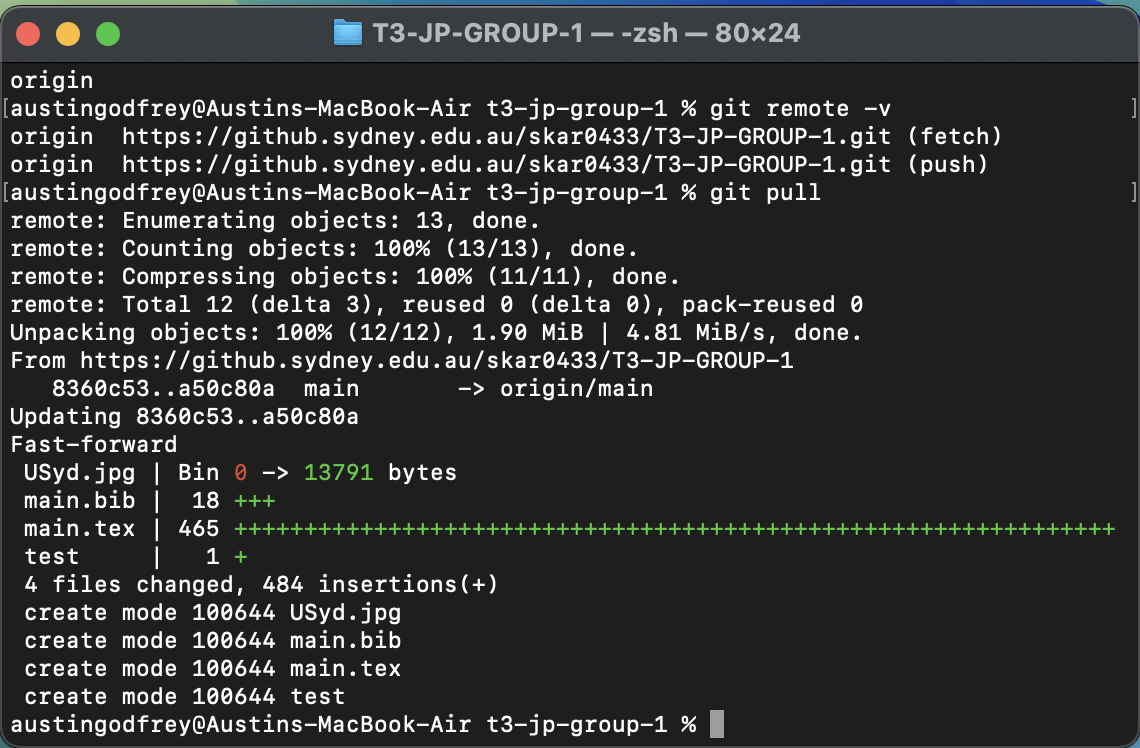
\includegraphics[width=0.8\textwidth]{git_pull}}
 \newline
 - Typed git pull in terminal to pull from the repo
\newline

\textbf{Pushing to git}
\newline



 1) Typed pdflatex main.tex in terminal to compile the LaTeX Document
 \newline
 \centering{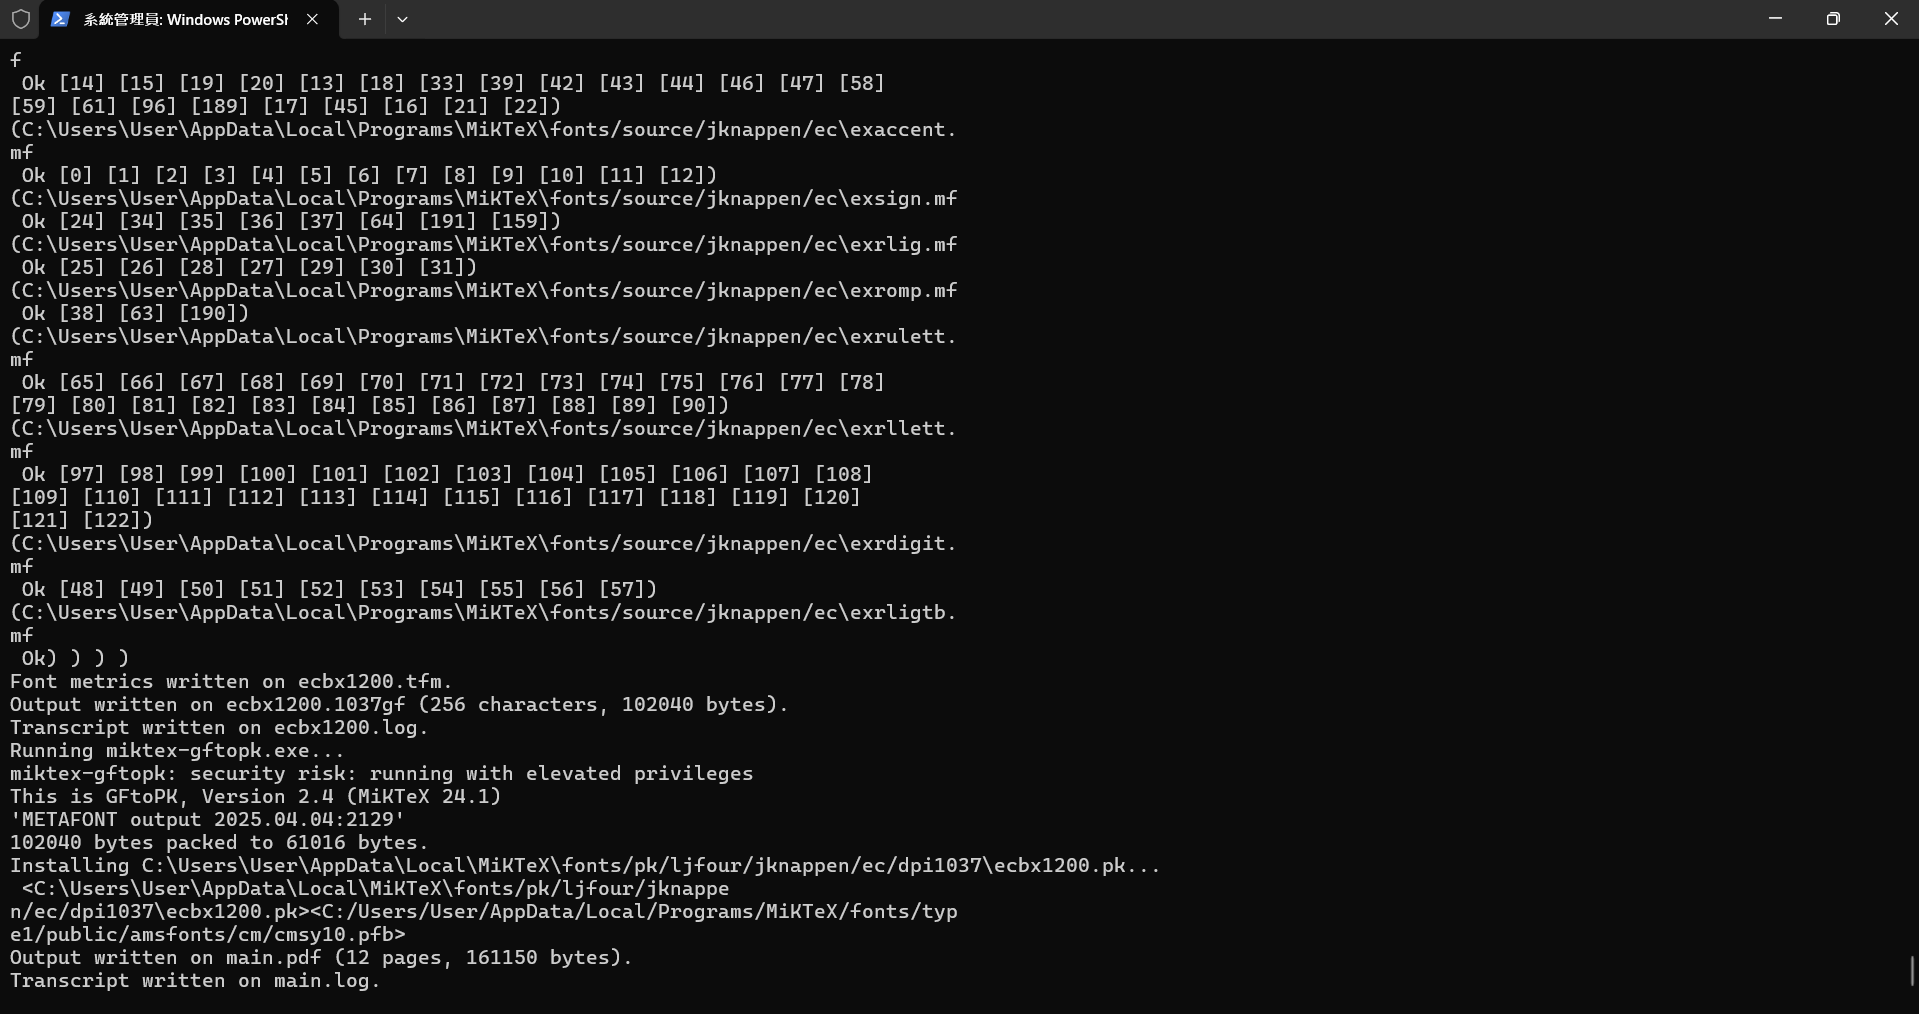
\includegraphics[width=0.8\textwidth]{pakopushfiles/compile.png}}

 \textbf{2) Used git commmit to commit the file to the main branch}
 \newline
 \centering{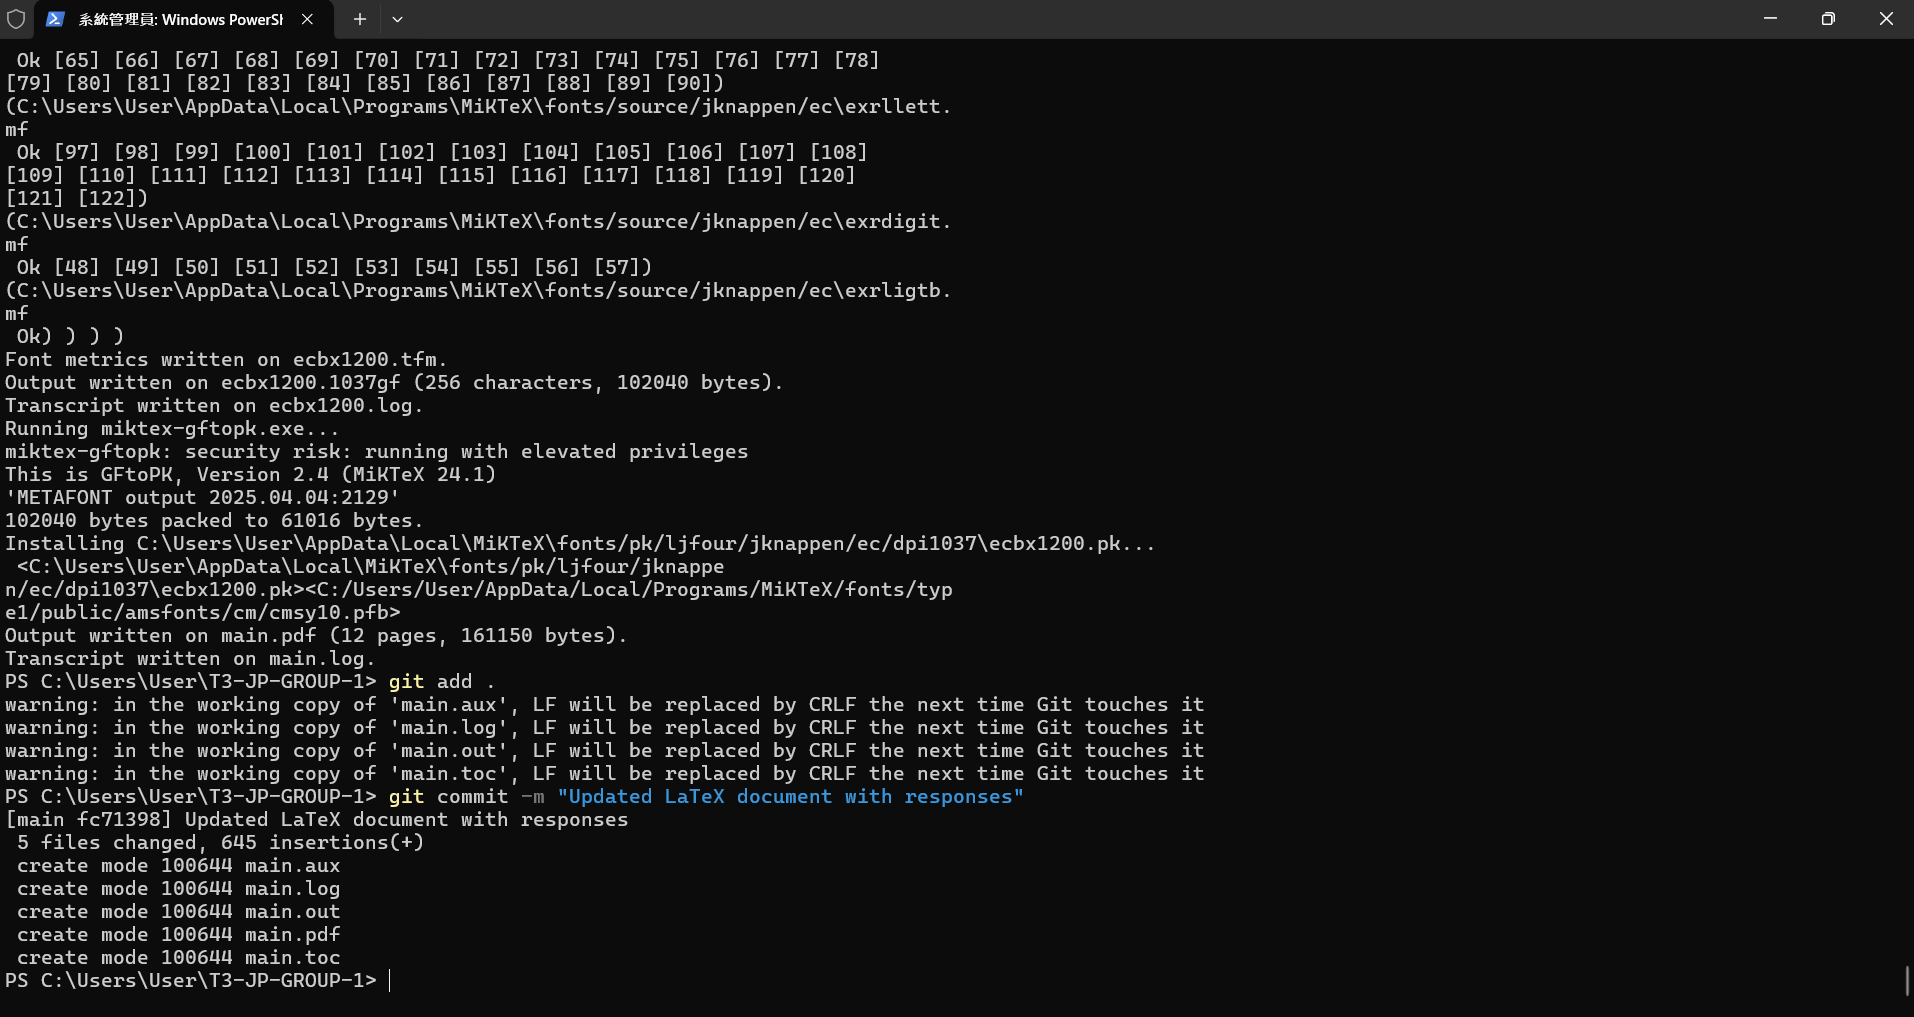
\includegraphics[width=0.8\textwidth]{pakopushfiles/commit_and_add.png}}

 3) Finally use git push to push the changes to the main branch
 \newline
 \centering{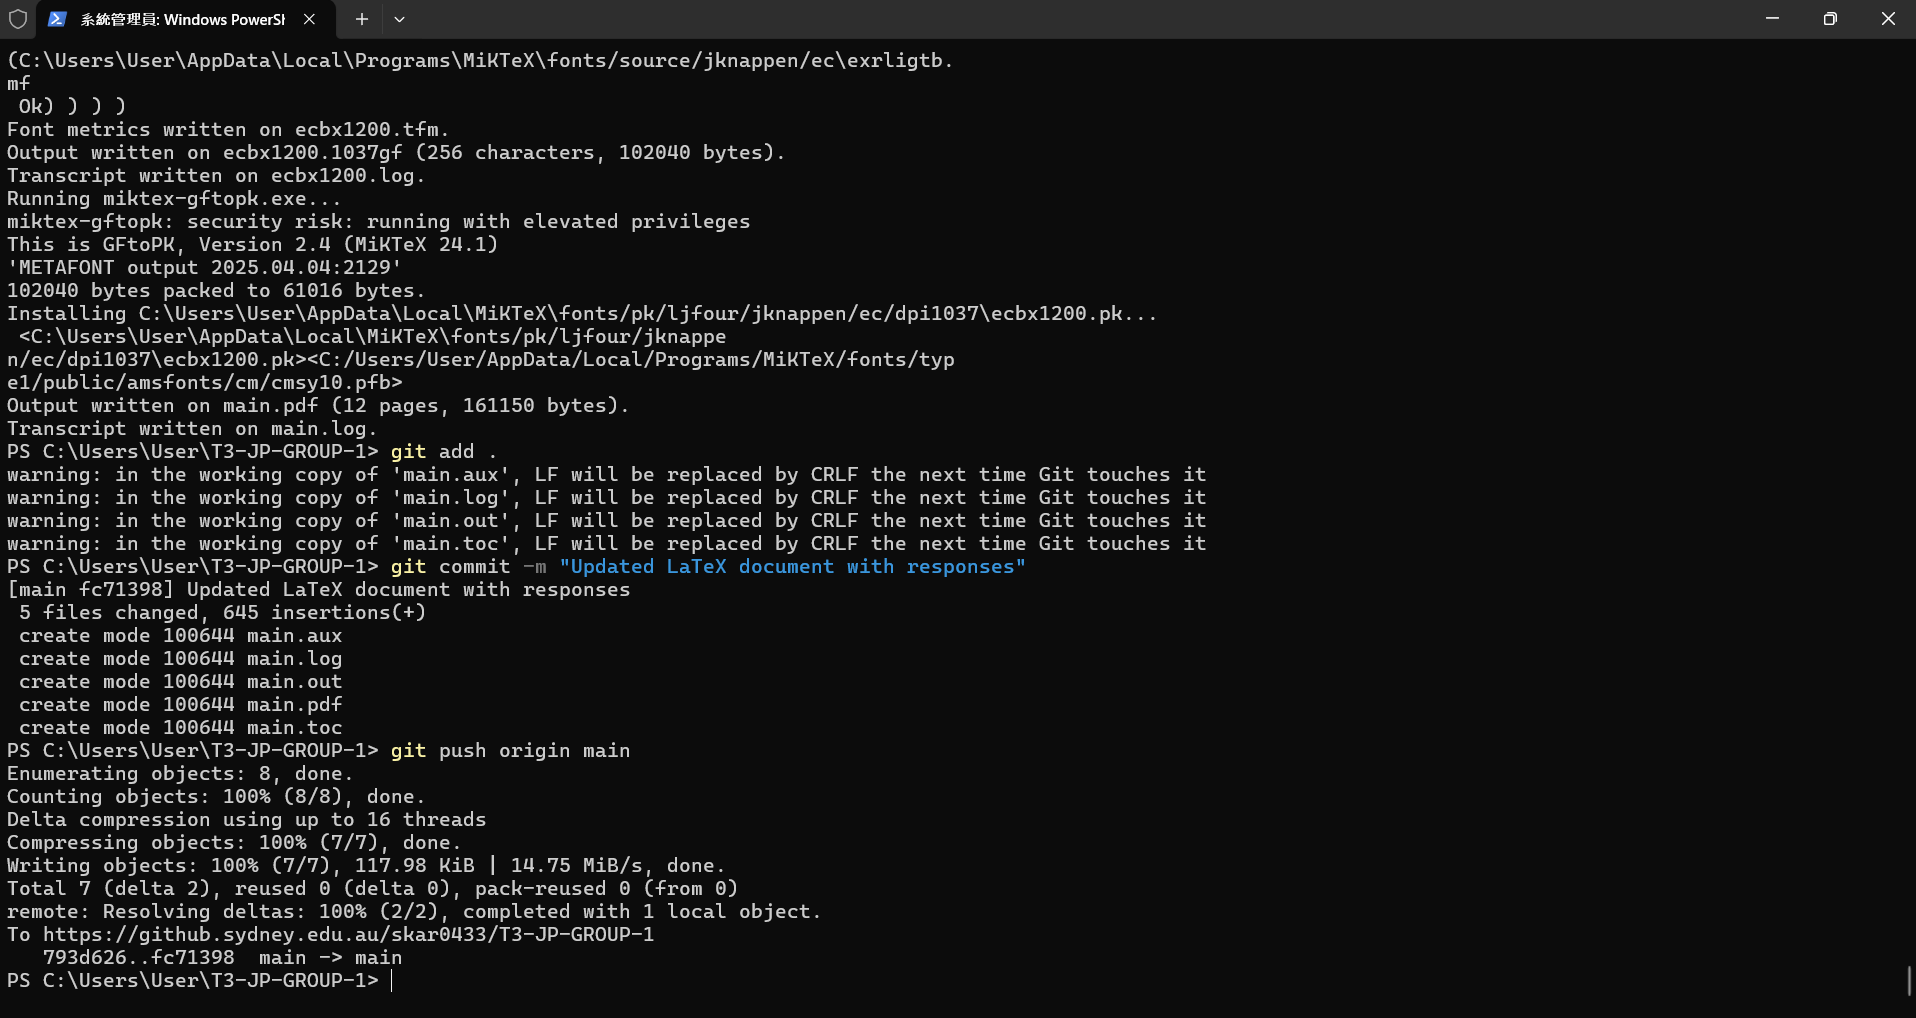
\includegraphics[width=0.8\textwidth]{pakopushfiles/push.png}}




\end{document}

